\documentclass{beamer}
\usetheme{jpal} % Use J-PAL theme
\setsansfont{Open Sans Light}
\setmonofont{Courier New}

\usepackage{booktabs}
\usepackage{pgfplots} % Not necessary. Used for graphs.
	\usepgfplotslibrary{dateplot}
	\usetikzlibrary{calc}
\usepackage{xspace} % Not necessary. Used for text macros.
	\newcommand{\jpalt}{\textbf{\textsc{J-PAL Theme}}\xspace}

\title{J-PAL Beamer Theme}
\subtitle{Rebranding comes to \LaTeX!}
\date{\today}
\author{Alvaro Carril}
\institute{Abdul Latif Jameel Poverty Action Lab}
\titlegraphic{\includegraphics[width=1.25in]{jpal_global}}

\begin{document}

\maketitle

%%%%%%%% INTRO %%%%%%%%%
\section{Introduction}

\begin{frame}{Motivation}
In 2016 J-PAL underwent a rebranding which greatly improves and unifies its identity. Although there is a well designed PowerPoint template accompanying this rebranding, \textbf{a LaTeX beamer template is missing}.

LaTeX presentations, under several circumstances, provide serious advantages over PowerPoint. However, LaTeX presentations' aesthetics are very outdated and difficult to customize. This theme aims to solve both issues, providing a \textbf{base template which already complies with the new guidelines} and also making it easy to tweak.
\end{frame}

\begin{frame}{Technical specifications and disclaimer}
The \jpalt theme is a LaTeX Beamer theme with minimal visual noise and designed to comply with J-PAL's latest rebranding guidelines. The theme is based on the \href{https://github.com/matze/mtheme}{\textit{Metropolis} Beamer Theme} by Matthias Vogelgesang.

Although it relies on XeLaTeX to compile using custom fonts, the theme can also be used with PDFLaTeX. It also requires a TikZ installation.
\end{frame}

\begin{frame}[fragile]{Using the theme}
\begin{itemize}
	\item This theme is simply a set of customizations on the \texttt{metropolis} beamer theme, which is included in the latest distributions of TeXLive and MiKTeX.
	\item If \texttt{metropolis} is installed, all that must be done is to place \texttt{jpaltheme.tex} in the same directory as your document. 
\end{itemize}

Enable the theme by loading
 \begin{verbatim}    \documentclass{beamer}
    \usetheme{metropolis}
    \input{jpaltheme}\end{verbatim}
\end{frame}

%%%%%%%% GUIDELINES %%%%%%%%%
\section{Guidelines Compliance}
\begin{frame}{Logo}
	\alert{J-PAL's new logo} can be easily inserted and positioned in the front page, as showcased in this presentation's first slide.
	\begin{itemize}
		\item Logos or other graphics can be easily included in the title slide using the \texttt{titlegraphic} command.
		\item The logo's width can be set in the \texttt{includegraphics} command. Proper spacing is already taken care of.
		\item More logos can be included by using \texttt{includegraphics} several times.
	\end{itemize}
\end{frame}

\begin{frame}{Colors}
	\alert{J-PAL's primary color palette} is already implemented in the theme.
	\begin{itemize}
		\item  All emphasized elements use \alert{J-PAL Red}, while some subtler visual elements use \textcolor{JPALteal}{J-PAL Teal}.
		\item The J-PAL color palette is fully implemented and its colors' names are as follows:
			\begin{itemize}
			\item \textcolor{JPALblack}{JPALblack}
			\item \textcolor{JPALred}{JPALred}
			\item \textcolor{JPALgreen}{JPALgreen}
			\item \textcolor{JPALyellow}{JPALyellow}
			\item \textcolor{JPALslate}{JPALslate}
			\item \textcolor{JPALteal}{JPALteal}
			\end{itemize}
	\end{itemize}
\end{frame}

\begin{frame}{Typography}
To use proper typography, several issues must be considered:
	\begin{itemize}
		\item In order to choose any system font, \alert{documents must be compiled with XeLaTeX}. 
		\item Open Sans font is freely available (this document was compiled with it), but recommended for \emph{web} use.
		\item The official typefaces, Futura and Mrs Eaves, are not available for free and don't come preinstalled in many OSs.
		\item If installed, this theme defaults to Mozilla's \emph{Fira Sans} fonts, which are also freely available on the web.
	\end{itemize}
If compiling with XeLaTeX, any font can be chosen with the \texttt{setsansfont} command in the preamble. See the \texttt{fontspec} package for more details.
\end{frame}


%%%%%%%% ELEMENTS %%%%%%%%%
\section{Elements}

\begin{frame}[fragile]{Introduction}
The following section showcases several usual LaTeX elements and how they are implemented in the \jpalt. It is mostly based on the original Demo developed by Matthias Vogelgesang.
\end{frame}

\begin{frame}[fragile]{Typography}
      \begin{verbatim}The theme provides sensible defaults to
\emph{emphasize} text, \alert{accent} parts
or show \textbf{bold} results.\end{verbatim}

  \begin{center}becomes\end{center}

  The theme provides sensible defaults to \emph{emphasize} text,
  \alert{accent} parts or show \textbf{bold} results.
\end{frame}

\begin{frame}{Font feature test}
Test if your loaded typeface has all these variations:
  \begin{itemize}
    \item Regular
    \item \textit{Italic}
    \item \textsc{SmallCaps}
    \item \textbf{Bold}
    \item \textbf{\textit{Bold Italic}}
    \item \textbf{\textsc{Bold SmallCaps}}
    \item \texttt{Monospace}
    \item \texttt{\textit{Monospace Italic}}
    \item \texttt{\textbf{Monospace Bold}}
    \item \texttt{\textbf{\textit{Monospace Bold Italic}}}
  \end{itemize}
\end{frame}

\begin{frame}{Lists}
Lists are indented for enhanced readability. This is consistent with J-PAL's Brand Guidelines.

\vspace{\baselineskip}
  \begin{columns}[T,onlytextwidth]
    \column{0.33\textwidth}
      Items
      \begin{itemize}
        \item Milk \item Eggs \item Potatos
      \end{itemize}

    \column{0.33\textwidth}
      Enumerations
      \begin{enumerate}
        \item First, \item Second and \item Last.
      \end{enumerate}

    \column{0.33\textwidth}
      Descriptions
      \begin{description}
        \item[PowerPoint] Meeh. \item[Beamer] Yeeeha.
      \end{description}
  \end{columns}
\end{frame}

\begin{frame}{References and footnotes}
Footnotes can be easily added.\footnote{This is a footnote.} References, on the other hand, follow LaTeX rules and conventions.
\end{frame}

\begin{frame}{Animation}
  \begin{itemize}[<+- | alert@+>]
    \item \alert<4>{This is\only<4>{ \emph{really}} important}
    \item Now this
    \item And now this
  \end{itemize}
\end{frame}

\begin{frame}{Figures}
  \begin{figure}
    \newcounter{density}
    \setcounter{density}{20}
    \begin{tikzpicture}
      \def\couleur{alerted text.fg}
      \path[coordinate] (0,0)  coordinate(A)
                  ++( 90:5cm) coordinate(B)
                  ++(0:5cm) coordinate(C)
                  ++(-90:5cm) coordinate(D);
      \draw[fill=\couleur!\thedensity] (A) -- (B) -- (C) --(D) -- cycle;
      \foreach \x in {1,...,40}{%
          \pgfmathsetcounter{density}{\thedensity+20}
          \setcounter{density}{\thedensity}
          \path[coordinate] coordinate(X) at (A){};
          \path[coordinate] (A) -- (B) coordinate[pos=.10](A)
                              -- (C) coordinate[pos=.10](B)
                              -- (D) coordinate[pos=.10](C)
                              -- (X) coordinate[pos=.10](D);
          \draw[fill=\couleur!\thedensity] (A)--(B)--(C)-- (D) -- cycle;
      }
    \end{tikzpicture}
    \caption{Rotated square from
    \href{http://www.texample.net/tikz/examples/rotated-polygons/}{texample.net}.}
  \end{figure}
\end{frame}

\begin{frame}{Text and figure side by side}
\begin{columns}[c]
    \begin{column}{.5\textwidth}
    \begin{itemize}
    	\item A perpendicular bisector of a line segment is a line which is perpendicular to this line and passes through its midpoint.
    	\item Figure \ref{fig:perpendicular_bisectors} shows perpendicular bisectors of a triangle.
    	\item Both bisectors meet in the center of the circumcircle of the triangle.	
    \end{itemize}
    \end{column}
	\begin{column}{.5\textwidth}
  \begin{figure}
  \scalebox{.6}{
    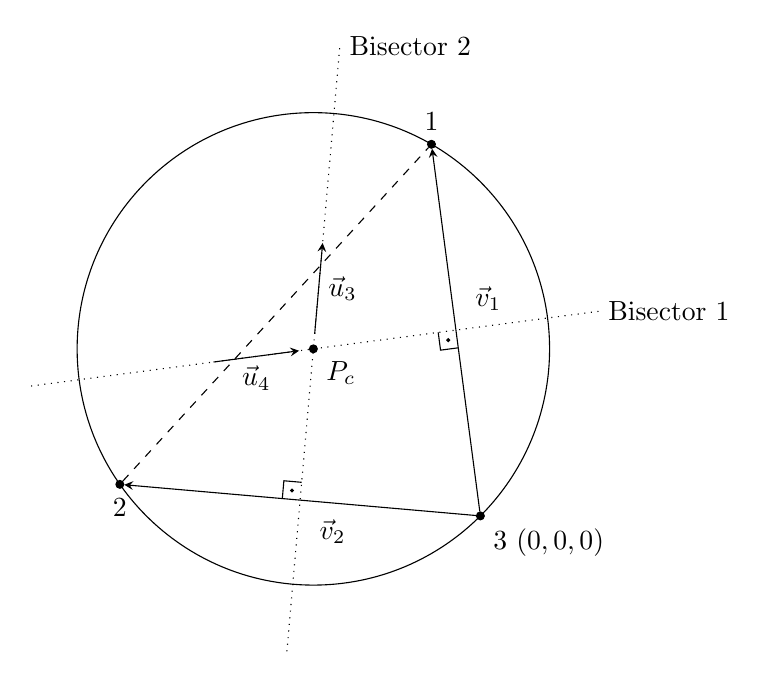
\begin{tikzpicture}
  [
    scale=3,
    >=stealth,
    point/.style = {draw, circle,  fill = black, inner sep = 1pt},
    dot/.style   = {draw, circle,  fill = black, inner sep = .2pt},
  ]

  % the circle
  \def\rad{1}
  \node (origin) at (0,0) [point, label = {below right:$P_c$}]{};
  \draw (origin) circle (\rad);

  % triangle nodes: just points on the circle
  \node (n1) at +(60:\rad) [point, label = above:$1$] {};
  \node (n2) at +(-145:\rad) [point, label = below:$2$] {};
  \node (n3) at +(-45:\rad) [point, label = {below right:$3$ $(0, 0, 0)$}] {};

  % triangle edges: connect the vertices, and leave a node at the midpoint
  \draw[->] (n3) -- node (a) [label = {above right:$\vec{v}_1$}] {} (n1);
  \draw[->] (n3) -- node (b) [label = {below right:$\vec{v}_2$}] {} (n2);
  \draw[dashed] (n2) -- (n1);

  % Bisectors
  % start at the point lying on the line from (origin) to (a), at
  % twice that distance, and then draw a path going to the point on
  % the line lying on the line from (a) to the (origin), at 3 times
  % that distance.
  \draw[dotted]
    ($ (origin) ! 2 ! (a) $)
    node [right] {Bisector 1}
    -- ($(a) ! 3 ! (origin)$ );

  % similarly for origin and b
  \draw[dotted]
    ($ (origin) ! 2 ! (b) $)
    -- ($(b) ! 3 ! (origin)$ )
    node [right] {Bisector 2};

  % short vectors
  \draw[->]
    ($ (origin) ! -.7 ! (a) $)
    -- node [below] {$\vec{u}_4$}
    ($ (origin) ! -.1 ! (a) $);
  \draw[->]
    ($ (origin) ! -.1 ! (b) $)
    -- node [right] {$\vec{u}_3$}
    ($ (origin) ! -.7 ! (b) $);

  % Right angle symbols
  \def\ralen{.5ex}  % length of the short segment
  \foreach \inter/\first/\last in {a/n3/origin, b/n2/origin}
    {
      \draw let \p1 = ($(\inter)!\ralen!(\first)$), % point along first path
                \p2 = ($(\inter)!\ralen!(\last)$),  % point along second path
                \p3 = ($(\p1)+(\p2)-(\inter)$)      % corner point
            in
              (\p1) -- (\p3) -- (\p2)               % path
              ($(\inter)!.5!(\p3)$) node [dot] {};  % center dot
    }
\end{tikzpicture}
}
	\caption{Perpendicular bisectors of a triangle from
    \href{http://www.texample.net/tikz/examples/rotated-polygons/}{texample.net}.}
    \label{fig:perpendicular_bisectors}
  \end{figure}
  \end{column}
  \end{columns}
\end{frame}

\begin{frame}{Tables}
  \begin{table}
    \caption{Largest cities in the world}
    \begin{tabular}{lr}
      \toprule
      City & Population\\
      \midrule
      Mexico City & 20,116,842\\
      Shanghai & 19,210,000\\
      Peking & 15,796,450\\
      Istanbul & 14,160,467\\
      \bottomrule
      \multicolumn{2}{l}{\footnotesize{\textit{Source:} Wikipedia}}
    \end{tabular}
  \end{table}
\end{frame}
\begin{frame}{Blocks}
  Three different block environments are pre-defined and may be styled with an
  optional background color.

  \begin{columns}[T,onlytextwidth]
    \column{0.5\textwidth}
      \begin{block}{Default}
        Block content.
      \end{block}

      \begin{alertblock}{Alert}
        Block content.
      \end{alertblock}

      \begin{exampleblock}{Example}
        Block content.
      \end{exampleblock}

    \column{0.5\textwidth}

      \metroset{block=fill}

      \begin{block}{Default}
        Block content.
      \end{block}

      \begin{alertblock}{Alert}
        Block content.
      \end{alertblock}

      \begin{exampleblock}{Example}
        Block content.
      \end{exampleblock}

  \end{columns}
\end{frame}
\begin{frame}{Math}
Of course, math typesets beautifully in LaTeX. Check out this elegant equation:
  \begin{equation*}
    e = \lim_{n\to \infty} \left(1 + \frac{1}{n}\right)^n .
  \end{equation*}
\end{frame}

\begin{frame}{Line plots}
  \begin{figure}
    \begin{tikzpicture}
      \begin{axis}[
        mlineplot,
        width=0.9\textwidth,
        height=6cm,
      ]

        \addplot {sin(deg(x))};
        \addplot+[samples=100] {sin(deg(2*x))};

      \end{axis}
    \end{tikzpicture}
  \end{figure}
\end{frame}

\begin{frame}{Bar charts}
  \begin{figure}
    \begin{tikzpicture}
      \begin{axis}[
        mbarplot,
        xlabel={Foo},
        ylabel={Bar},
        width=0.9\textwidth,
        height=6cm,
      ]

      \addplot plot coordinates {(1, 20) (2, 25) (3, 22.4) (4, 12.4)};
      \addplot plot coordinates {(1, 18) (2, 24) (3, 23.5) (4, 13.2)};
      \addplot plot coordinates {(1, 10) (2, 19) (3, 25) (4, 15.2)};

      \legend{lorem, ipsum, dolor}

      \end{axis}
    \end{tikzpicture}
  \end{figure}
\end{frame}
\begin{frame}{Quotes}
  \begin{quote}
    I seek not to know the answers, but to understand the questions.
  \end{quote}
\end{frame}


\plain{¡Thank you!\\[1cm]\small Please email comments or suggestions to \url{acarril@povertyactionlab.org}}

\end{document}